%% This is file `elsarticle-template-1-num.tex',
%%
%% Copyright 2009 Elsevier Ltd
%%
%% This file is part of the 'Elsarticle Bundle'.
%% ---------------------------------------------
%%
%% It may be distributed under the conditions of the LaTeX Project Public
%% License, either version 1.2 of this license or (at your option) any
%% later version.  The latest version of this license is in
%%    http://www.latex-project.org/lppl.txt
%% and version 1.2 or later is part of all distributions of LaTeX
%% version 1999/12/01 or later.
%%
%% Template article for Elsevier's document class `elsarticle'
%% with numbered style bibliographic references
%%
%% $Id: elsarticle-template-1-num.tex 149 2009-10-08 05:01:15Z rishi $
%% $URL: http://lenova.river-valley.com/svn/elsbst/trunk/elsarticle-template-1-num.tex $
%%
\documentclass[preprint,12pt]{elsarticle}

%% Use the option review to obtain double line spacing
%% \documentclass[preprint,review,12pt]{elsarticle}

%% Use the options 1p,twocolumn; 3p; 3p,twocolumn; 5p; or 5p,twocolumn
%% for a journal layout:
%% \documentclass[final,1p,times]{elsarticle}
%% \documentclass[final,1p,times,twocolumn]{elsarticle}
%% \documentclass[final,3p,times]{elsarticle}
%% \documentclass[final,3p,times,twocolumn]{elsarticle}
%% \documentclass[final,5p,times]{elsarticle}
%% \documentclass[final,5p,times,twocolumn]{elsarticle}

%% The graphicx package provides the includegraphics command.
\usepackage{graphicx}
%% The amssymb package provides various useful mathematical symbols
\usepackage{amssymb}
%% The amsthm package provides extended theorem environments
%% \usepackage{amsthm}

%% The lineno packages adds line numbers. Start line numbering with
%% \begin{linenumbers}, end it with \end{linenumbers}. Or switch it on
%% for the whole article with \linenumbers after \end{frontmatter}.
\usepackage{lineno}

%% natbib.sty is loaded by default. However, natbib options can be
%% provided with \biboptions{...} command. Following options are
%% valid:

%%   round  -  round parentheses are used (default)
%%   square -  square brackets are used   [option]
%%   curly  -  curly braces are used      {option}
%%   angle  -  angle brackets are used    <option>
%%   semicolon  -  multiple citations separated by semi-colon
%%   colon  - same as semicolon, an earlier confusion
%%   comma  -  separated by comma
%%   numbers-  selects numerical citations
%%   super  -  numerical citations as superscripts
%%   sort   -  sorts multiple citations according to order in ref. list
%%   sort&compress   -  like sort, but also compresses numerical citations
%%   compress - compresses without sorting
%%
%% \biboptions{comma,round}

% \biboptions{}

\journal{Journal Name}

\begin{document}

\begin{frontmatter}

%% Title, authors and addresses

\title{Unnecessarily Complicated Research Title}

%% use the tnoteref command within \title for footnotes;
%% use the tnotetext command for the associated footnote;
%% use the fnref command within \author or \address for footnotes;
%% use the fntext command for the associated footnote;
%% use the corref command within \author for corresponding author footnotes;
%% use the cortext command for the associated footnote;
%% use the ead command for the email address,
%% and the form \ead[url] for the home page:
%%
%% \title{Title\tnoteref{label1}}
%% \tnotetext[label1]{}
%% \author{Name\corref{cor1}\fnref{label2}}
%% \ead{email address}
%% \ead[url]{home page}
%% \fntext[label2]{}
%% \cortext[cor1]{}
%% \address{Address\fnref{label3}}
%% \fntext[label3]{}


%% use optional labels to link authors explicitly to addresses:
%% \author[label1,label2]{<author name>}
%% \address[label1]{<address>}
%% \address[label2]{<address>}

\author{John Smith}

\address{California, United States}

\begin{abstract}
%% Text of abstract
Suspendisse potenti. Suspendisse quis sem elit, et mattis nisl. Phasellus consequat erat eu velit rhoncus non pharetra neque auctor. Phasellus eu lacus quam. Ut ipsum dolor, euismod aliquam congue sed, lobortis et orci. Mauris eget velit id arcu ultricies auctor in eget dolor. Pellentesque suscipit adipiscing sem, imperdiet laoreet dolor elementum ut. Mauris condimentum est sed velit lacinia placerat. Vestibulum ante ipsum primis in faucibus orci luctus et ultrices posuere cubilia Curae; Nullam diam metus, pharetra vitae euismod sed, placerat ultrices eros. Aliquam tincidunt dapibus venenatis. In interdum tellus nec justo accumsan aliquam. Nulla sit amet massa augue.
\end{abstract}

\begin{keyword}
Science \sep Publication \sep Complicated
%% keywords here, in the form: keyword \sep keyword

%% MSC codes here, in the form: \MSC code \sep code
%% or \MSC[2008] code \sep code (2000 is the default)

\end{keyword}

\end{frontmatter}

%%
%% Start line numbering here if you want
%%
\linenumbers

%% main text
\section{The First Section}
\label{S:1}

Maecenas urna ac sapien tincidunt lobortis. Nunc feugiat faucibus varius. Ut sed purus nunc. Ut eget eros quis lectus mollis pharetra ut in tellus. Pellentesque ultricies velit sed orci pharetra et fermentum lacus imperdiet. Class aptent taciti sociosqu ad litora torquent per conubia nostra, per inceptos himenaeos. Suspendisse commodo ultrices mauris, condimentum hendrerit lorem condimentum et. Pellentesque urna augue, semper et rutrum ac, consequat id quam. Proin lacinia aliquet justo, ut suscipit massa commodo sit amet. Proin vehicula nibh nec mauris tempor interdum. Donec orci ante, tempor a viverra vel, volutpat sed orci.

\begin{itemize}
\item Bullet point one
\item Bullet point two
\end{itemize}

\begin{enumerate}
\item Numbered list item one
\item Numbered list item two
\end{enumerate}

\subsection{Subsection One}

Quisque elit ipsum, porttitor et imperdiet in, facilisis ac diam. Nunc facilisis interdum felis eget tincidunt. In condimentum fermentum leo, non consequat leo imperdiet pharetra. Fusce ac massa ipsum, vel convallis diam. Quisque eget turpis felis. Curabitur posuere, risus eu placerat porttitor, magna metus mollis ipsum, eu volutpat nisl erat ac justo. Nullam semper, mi at iaculis viverra, nunc velit iaculis nunc, eu tempor ligula eros in nulla. Aenean dapibus eleifend convallis. Cras ut libero tellus. Integer mollis eros eget risus malesuada fringilla mattis leo facilisis. Etiam interdum turpis eget odio ultricies sed convallis magna accumsan. Morbi in leo a mauris sollicitudin molestie at non nisl.

\begin{table}[h]
\centering
\begin{tabular}{l l l}
\hline
\textbf{Treatments} & \textbf{Response 1} & \textbf{Response 2}\\
\hline
Treatment 1 & 0.0003262 & 0.562 \\
Treatment 2 & 0.0015681 & 0.910 \\
Treatment 3 & 0.0009271 & 0.296 \\
\hline
\end{tabular}
\caption{Table caption}
\end{table}

\subsection{Subsection Two}


\begin{figure}[h]
\centering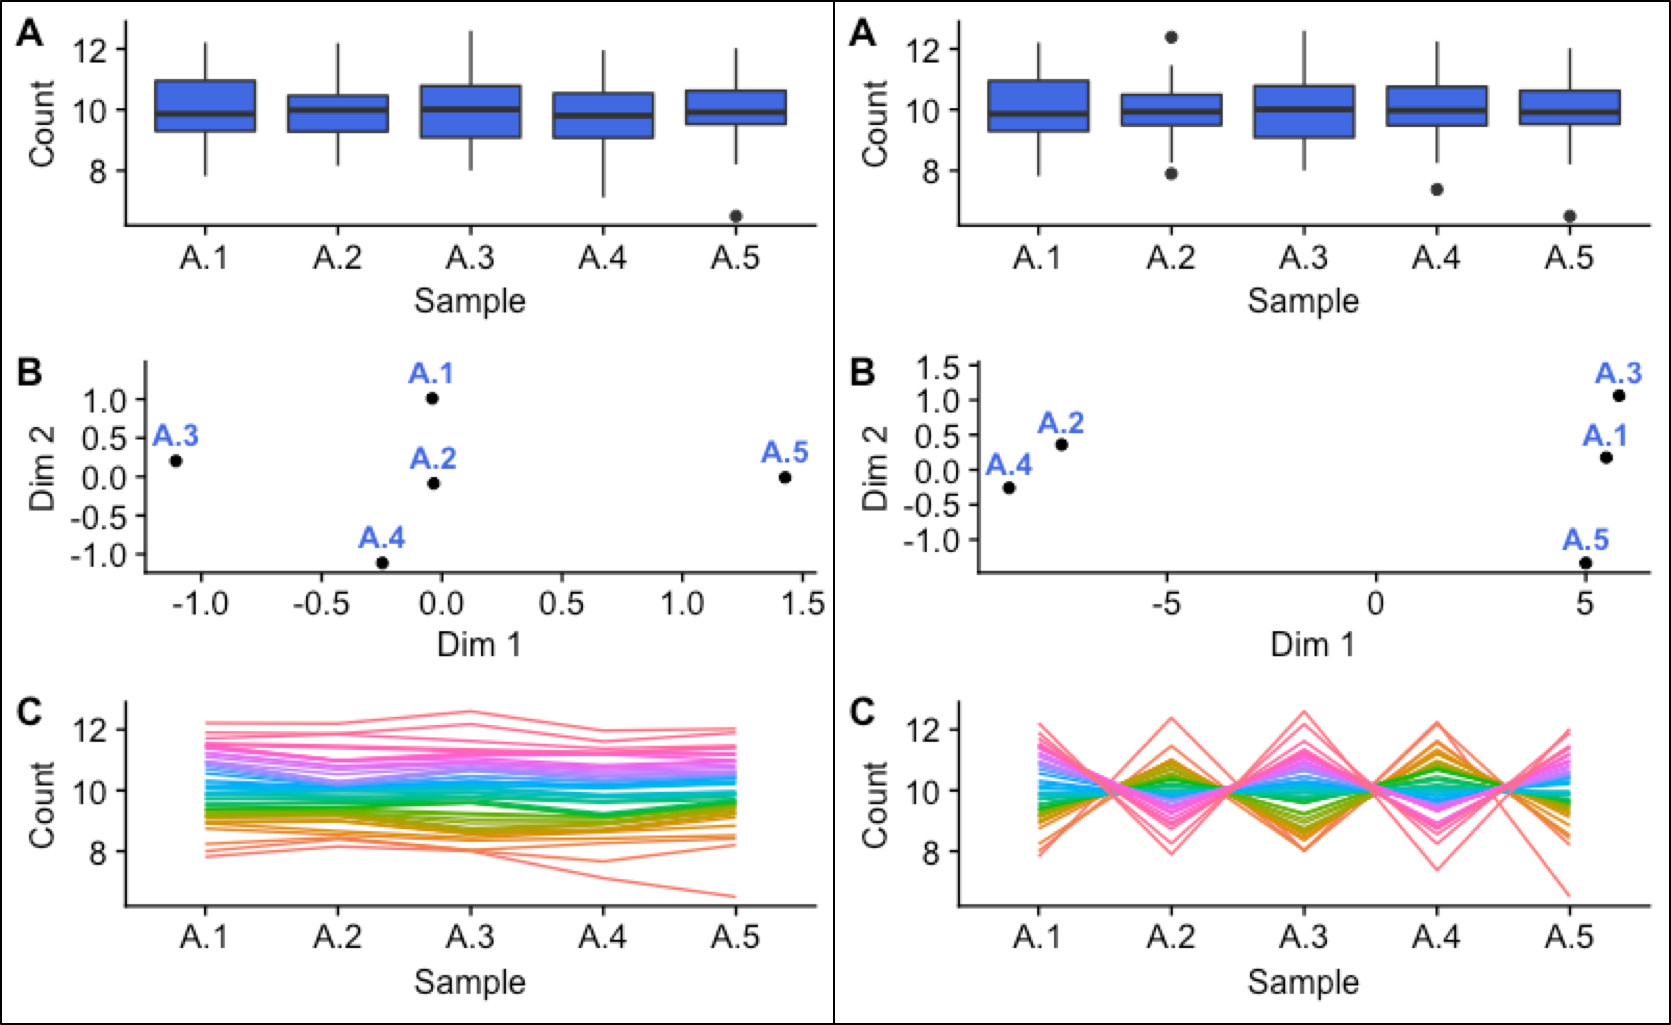
\includegraphics[width=\linewidth]{/Users/lindz/JDSPaper/Bioinformatics/Pictures/bmp/Color/1group.png}
\caption{Caption}
\end{figure}

\begin{figure}[h]
\centering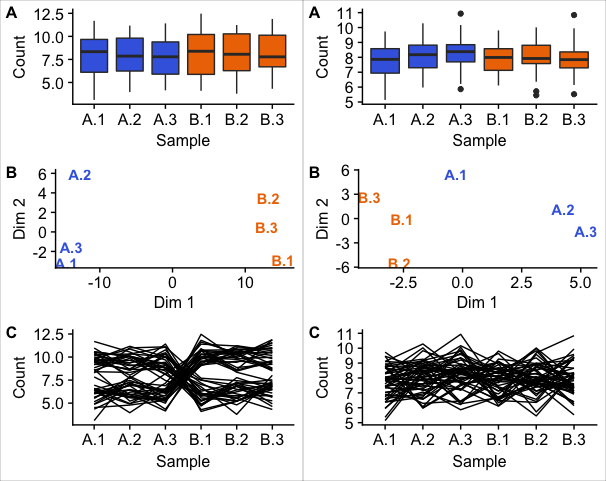
\includegraphics[width=\linewidth]{/Users/lindz/JDSPaper/Bioinformatics/Pictures/bmp/Color/2group.png}
\caption{Caption}
\end{figure}

\begin{figure}[h]
\centering\includegraphics[width=\linewidth]{/Users/lindz/JDSPaper/Bioinformatics/Pictures/SwitchSample/Switch12/NotSwitch/S1_S2_10hex.jpg}
\caption{Caption}
\end{figure}

\begin{figure}[h]
\centering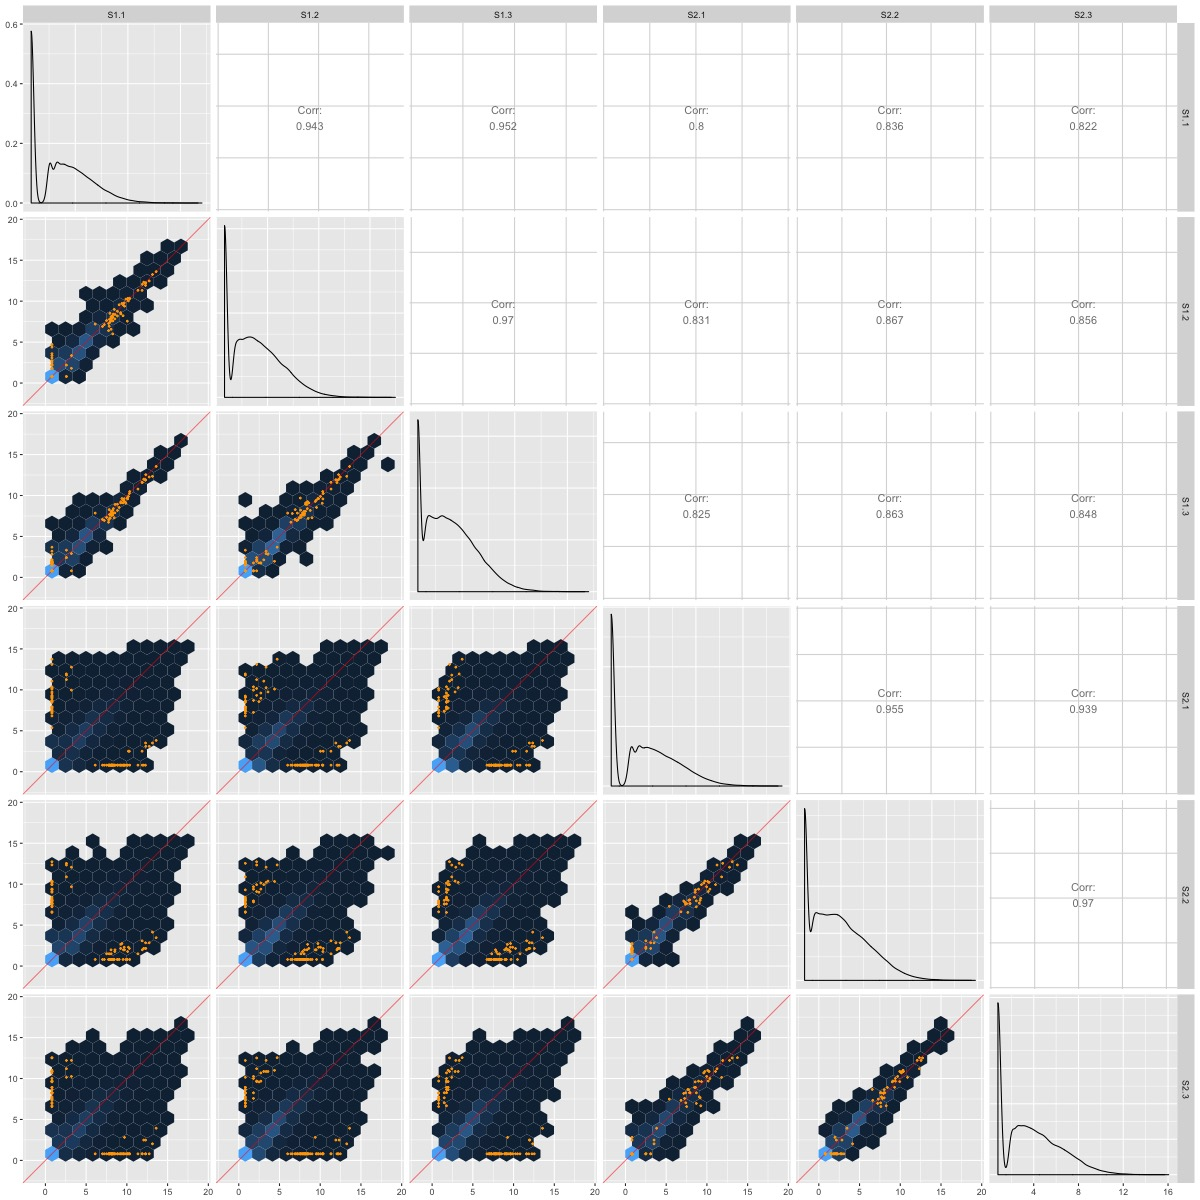
\includegraphics[width=\linewidth]{{/Users/lindz/JDSPaper/Bioinformatics/Pictures/SwitchSample/Switch12/NotSwitch/S1_S2_deg_sm_0.05}.jpg}
\caption{Caption}
\end{figure}

\begin{figure}[h]
\centering\includegraphics[width=\linewidth]{/Users/lindz/JDSPaper/Bioinformatics/Pictures/SwitchSample/Switch12/Switched/S1_S2_10hex.jpg}
\caption{Caption}
\end{figure}

Below shows not switched followed by switched

\begin{figure}[h]
\centering\includegraphics[width=0.5\linewidth]{/Users/lindz/JDSPaper/Bioinformatics/Pictures/SwitchSample/Switch12/NotSwitch/MDS.png}
\caption{Caption}
\end{figure}

\begin{figure}[h]
\centering\includegraphics[width=0.5\linewidth]{/Users/lindz/JDSPaper/Bioinformatics/Pictures/SwitchSample/Switch12/Switched/MDS.png}
\caption{Caption}
\end{figure}

\begin{figure}[h]
\centering\includegraphics[width=0.5\linewidth]{{/Users/lindz/JDSPaper/Bioinformatics/Pictures/SwitchSample/Switch12/NotSwitch/S1_S2_deg_pcp_0.05}.jpg}
\caption{Caption}
\end{figure}

\begin{figure}[h]
\centering\includegraphics[width=0.5\linewidth]{{/Users/lindz/JDSPaper/Bioinformatics/Pictures/SwitchSample/Switch12/Switched/S1_S2_deg_pcp_0.05}.jpg}
\caption{Caption}
\end{figure}

\begin{figure}[h]
\centering\includegraphics[width=0.5\linewidth]{/Users/lindz/JDSPaper/Bioinformatics/Pictures/SwitchSample/Switch12/NotSwitch/S1_S2_deg_volcano.jpg}
\caption{Caption}
\end{figure}

\begin{figure}[h]
\centering\includegraphics[width=0.5\linewidth]{/Users/lindz/JDSPaper/Bioinformatics/Pictures/SwitchSample/Switch12/Switched/S1_S2_deg_volcano.jpg}
\caption{Caption}
\end{figure}

Below shows raw followed by TMM

\begin{figure}[h]
\centering\includegraphics[width=\linewidth]{/Users/lindz/JDSPaper/Bioinformatics/Pictures/liverKidney/raw/R1/K_L_10hex.jpg}
\caption{Caption}
\end{figure}

\begin{figure}[h]
\centering\includegraphics[width=\linewidth]{/Users/lindz/JDSPaper/Bioinformatics/Pictures/liverKidney/tmmNorm/R1/K_L_10hex.jpg}
\caption{Caption}
\end{figure}

\begin{figure}[h]
\centering\includegraphics[width=0.5\linewidth]{/Users/lindz/JDSPaper/Bioinformatics/Pictures/liverKidney/raw/MDS.png}
\caption{Caption}
\end{figure}

\begin{figure}[h]
\centering\includegraphics[width=0.5\linewidth]{/Users/lindz/JDSPaper/Bioinformatics/Pictures/liverKidney/tmmNorm/MDS.png}
\caption{Caption}
\end{figure}

\begin{figure}[h]
\centering\includegraphics[width=0.5\linewidth]{/Users/lindz/JDSPaper/Bioinformatics/Pictures/liverKidney/raw/R1/boxplot.jpg}
\caption{Caption}
\end{figure}

\begin{figure}[h]
\centering\includegraphics[width=0.5\linewidth]{/Users/lindz/JDSPaper/Bioinformatics/Pictures/liverKidney/tmmNorm/R1/boxplot.jpg}
\caption{Caption}
\end{figure}

Raw followed by betweenLane

\begin{figure}[h]
\centering\includegraphics[width=\linewidth]{/Users/lindz/JDSPaper/Data/risso-Yeast/raw/Y1_Y4_points.jpg}
\caption{Caption}
\end{figure}

\begin{figure}[h]
\centering\includegraphics[width=\linewidth]{/Users/lindz/JDSPaper/Data/risso-Yeast/between/Y1_Y4_points.jpg}
\caption{Caption}
\end{figure}

\begin{figure}[h]
\centering\includegraphics[width=0.5\linewidth]{/Users/lindz/JDSPaper/Bioinformatics/Pictures/yeast/raw/MDS.png}
\caption{Caption}
\end{figure}

\begin{figure}[h]
\centering\includegraphics[width=0.5\linewidth]{/Users/lindz/JDSPaper/Bioinformatics/Pictures/yeast/between/MDS.png}
\caption{Caption}
\end{figure}

\begin{figure}[h]
\centering\includegraphics[width=0.5\linewidth]{/Users/lindz/JDSPaper/Bioinformatics/Pictures/yeast/raw/boxplot.jpg}
\caption{Caption}
\end{figure}

\begin{figure}[h]
\centering\includegraphics[width=0.5\linewidth]{/Users/lindz/JDSPaper/Bioinformatics/Pictures/yeast/between/boxplot.jpg}
\caption{Caption}
\end{figure}

\begin{figure}[h]
\centering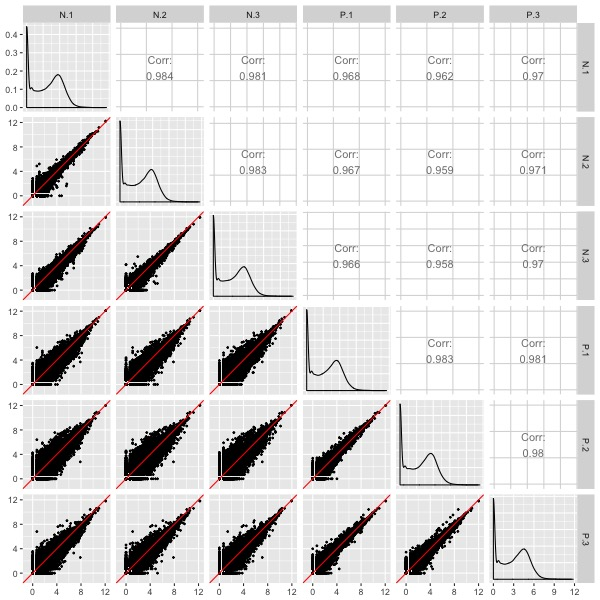
\includegraphics[width=\linewidth]{/Users/lindz/JDSPaper/Bioinformatics/Pictures/soybeanStreak/N_P_points.jpg}
\caption{Caption}
\end{figure}

\begin{figure}[h]
\centering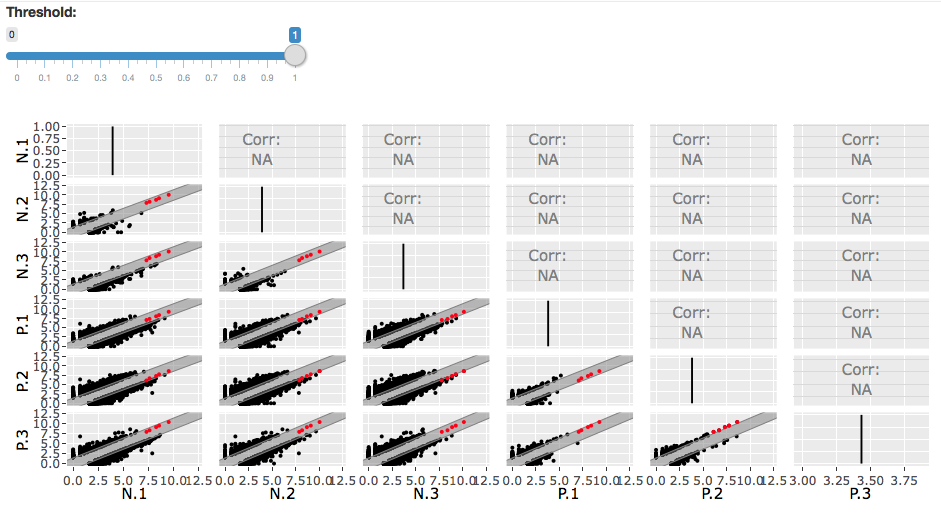
\includegraphics[width=\linewidth]{/Users/lindz/Desktop/findStreak1.png}
\caption{Caption}
\end{figure}

\begin{figure}[h]
\centering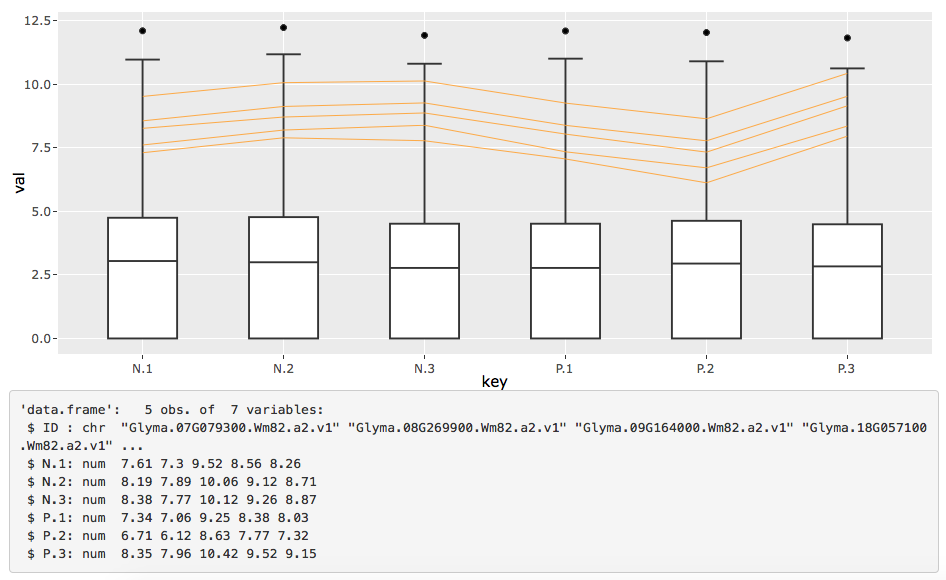
\includegraphics[width=\linewidth]{/Users/lindz/Desktop/findStreak2.png}
\caption{Caption}
\end{figure}


\section{The Second Section}
\label{S:2}

Reference to Section \ref{S:1}. Etiam congue sollicitudin diam non porttitor. Etiam turpis nulla, auctor a pretium non, luctus quis ipsum. Fusce pretium gravida libero non accumsan. Donec eget augue ut nulla placerat hendrerit ac ut mi. Phasellus euismod ornare mollis. Proin tempus fringilla ultricies. Donec pretium feugiat libero quis convallis. Nam interdum ante sed magna congue eu semper tellus sagittis. Curabitur eu augue elit.


%% The Appendices part is started with the command \appendix;
%% appendix sections are then done as normal sections
%% \appendix

%% \section{}
%% \label{}

%% References
%%
%% Following citation commands can be used in the body text:
%% Usage of \cite is as follows:
%%   \cite{key}          ==>>  [#]
%%   \cite[chap. 2]{key} ==>>  [#, chap. 2]
%%   \citet{key}         ==>>  Author [#]

%% References with bibTeX database:

\bibliographystyle{model1-num-names}
\bibliography{sample.bib}

%% Authors are advised to submit their bibtex database files. They are
%% requested to list a bibtex style file in the manuscript if they do
%% not want to use model1-num-names.bst.

%% References without bibTeX database:

% \begin{thebibliography}{00}

%% \bibitem must have the following form:
%%   \bibitem{key}...
%%

% \bibitem{}

% \end{thebibliography}


\end{document}

%%
%% End of file `elsarticle-template-1-num.tex'.